\documentclass{article}
\usepackage{fullpage}
\usepackage{color}
\usepackage[normalem]{ulem}
\newcommand{\eric}{\textcolor{blue}{[Eric]}}
\newcommand{\richard}{\textcolor{red}{[Richard]}}
\newcommand{\taylor}{\textcolor{green}{[Taylor]}}
\newcommand{\susi}{\textcolor{cyan}{[Susi]}}
\hyphenpenalty=100000
\usepackage{graphicx}
\DeclareGraphicsExtensions{.pdf,.png,.jpg}
\begin{document}
\setlength{\voffset}{3.5in}
\title{Milestone 2}
\author{Team Sriram\\
(Susi Cisneros, Eric Henderson, Taylor Purviance and Richard Thai)}
\date{7 October 2011}
\maketitle
\clearpage
\setlength{\voffset}{0pt}
\tableofcontents
\clearpage
~\\
\begin{Large}\textbf{Changes (based off Git commits)}\end{Large}\\
~\\
\begin{tabular}{ | p{2in} | p{4.5in} | }
\hline
\textbf{Date Time} & \textbf{Description}\\
\hline
\hline
\end{tabular}
\clearpage

\section{Executive Summary}
This milestone, the second of a series, documents the context for a software project proposed by the client, Tim Ekl. This document also keeps track of the use cases involved with the final product which include adding an item, basic searching, advanced searching, sorting search results, viewing item details, editing item details, and generating inventory reports. All of the use cases satisfy a set of features and keep track of actors, basic/alternative flow of events, pre-conditions, post-conditions, extension points, and special requirements. In addition, this document storyboards the final product as well as keep track of the context/data flow diagrams.

\section{Introduction}
TODO: \richard

\section{User Environment}
\begin{itemize}
\item The client uses Chrome whenever possible and prefers that development support Chrome and Firefox browsers.
\item The final product should operate on a Linux server with standard programming languages, programming frameworks, and Apache.  Additional packages can be installed if necessary.
\end{itemize}

\section{User Needs}
\begin{tabular}{ | p{0.15in} | p{4.0in} | p{.75in} |}
\hline
\textbf{ID} & \textbf{Need} & \textbf{Priority} \\
\hline
\hline
N0 & Search for parts based off their attributes & Primary \\
\hline
N1 & Identify items via bar codes & Primary \\
\hline
N2 & Keep track of the data associated with an asset & Primary \\
\hline
N3 & Organize search results & Primary \\
\hline
N4 & Insert objects in the system at any point; do not freeze the database & Secondary \\
\hline
N5 & Modify objects; including adding notes to the objects & Secondary \\
\hline
N6 & Access from a second physical location & Optional \\
\hline
N7 & View most-recently acquired asset(s) & Optional \\
\hline
N8 & View a summary of inventory data & Optional \\
\hline
\end{tabular}

\section{Features}
\subsection{Feature Listing}
\begin{tabular}{ | p{0.15in} | p{2.0in} | p{0.5in} | p{0.5in} | p{0.5in} | p{0.6in} | p{0.5in} | p{0.65in} | }
\hline
\textbf{ID} & \textbf{Feature} & \textbf{Priority} & \textbf{Effort} & \textbf{Risk} & \textbf{Stability} & \textbf{Target Release} & \textbf{Assigned To} \\
\hline
\hline
F0 & Online UI & Critical & High & High & Low & 1.0 & Eric \\
\hline
F1 & Add assets to the inventory & Critical & Low & High & Low & 1.0 & Richard \\
\hline
F2 & Modify assets in the inventory & Critical & Low & High & Low & 1.0 & Taylor \\
\hline
F3 & The system keeps track of attributes based on category & Critical & Low & High & Low & 1.0 & Susi \\
\hline
F4 & Use a UPC-A barcode as the unique identifier for each asset & Critical & Low & Medium & Low & 1.0 & Eric \\
\hline
F5 & Provide an updated list of recently-added assets & Useful & Medium & Low & Medium & 1.5 & Richard \\
\hline
F6 & Generate reports of asset inventory & Useful & High & Low & Medium & 2.0 & Taylor \\
\hline
F7 & Sort search results based off of barcode, title, and modified/created timestamp & Useful & High & Low & Low & 2.0 & Susi \\
\hline
F8 & Basic search for items based on name or UPC & Critical & High & High & Low & 1.0 & Eric \\
\hline
F9 & Advanced search for items based on all fields related to the item and its category & Critical & High & High & Low & 1.0 & Richard \\
\hline
F10 & Basic and Advanced searches allow the user to include wildcards in the query & Critical & High & High & Low & 1.0 & Taylor \\
\hline
F11 & Basic and Advanced searches will search first by exact/wildcard match, then by fuzzy match & Critical & High & High & Low & 1.0 & Susi \\
\hline
F12 & REST API & Critical & High & High & Low & 1.0 & Eric \\
\hline
\end{tabular}\\
~\\
~\\
\subsection{Feature-to-Need Correspondence}
\begin{tabular}{ | c || c | c | c | c | c | c | c | c | c | c | }
\hline
    & N0 & N1 & N2 & N3 & N4 & N5 & N6 & N7 & N8 \\
\hline
\hline
F0  &    &    &    &    &    &    & X  &    &    \\
\hline
F1  &    &    & X  &    & X  &    &    &    &    \\
\hline
F2  &    &    & X  &    &    & X  &    &    &    \\
\hline
F3  &    &    & X  &    & X  & X  &    &    &    \\
\hline
F4  & X  & X  & X  &    &    &    &    &    &    \\
\hline
F5  &    &    &    &    &    &    &    & X  &    \\
\hline
F6  &    &    &    &    &    &    &    &    & X  \\
\hline
F7  & X  & X  &    & X  &    &    &    &    &    \\
\hline
F8  & X  & X  & X  & X  &    &    &    &    &    \\
\hline
F9  & X  & X  & X  & X  &    &    &    &    &    \\
\hline
F10 & X  & X  & X  & X  &    &    &    &    &    \\
\hline
F11 & X  & X  & X  & X  &    &    &    &    &    \\
\hline
F12 &    &    &    &    &    &    & X  &    &    \\
\hline
\end{tabular}

\section{Client Background}
Tim Ekl is a Rose-Hulman graduate student who possesses a significant amount of computer hardware.  He plans on using this system to be able to quickly and easily locate the equipment he wants to use.  Tim is an experienced developer and plans on maintaining the system after it is finished.  

\section{Current System}
The client does not have a software solution in place.  Currently, Tim has a primitive categorization system in place which involves labeling boxes and then trying to deduce the location of a desired component.  The current system poses a few issues such as not always allowing him to find his items, i.e. there have been instances where an item was found after capital was spent to replace it.

\section{Project Background}
TODO: \richard

\section{Use Cases}

\paragraph{Use case syntax}\\
~\\
Each use case is divided into 8 sections:
\begin{itemize}
\item A “Basic Description” section which gives an overview of what functionality the use case demonstrates.
\item An “Actors” section to describe who or what interacts with the system in the use case.
\item A “Pre-conditions” section which contains the assumptions made, especially those pertaining to the state of the system, prior to the start of the use case.
\item A “Basic Flow of Events” section which details the order of events done by the actor(s) and the system under standard conditions. If a particular step in the basic flow has the possibility of failing to occur successfully, one or more alternative flow listings are presented in brackets following the possibility of failure. Each alternative flow listing matches to an alternative flow in the “Alternative Flow” section. If a basic flow step fails, the alternative flow that is listed with it is followed as the next step.
\item An “Alternative Flow of Events” section which holds each alternative flow listed in the basic flow. Each alternative flow has a unique identifier used to reference it, a short name describing the condition that would cause the alternative flow to be followed, and the order of actions performed by the actor(s) and the system under the flow’s conditions. If an action has the possibility of failing, alternatives to that flow are presented just as they are in the basic flow with a reference to the alternative flow to take.
\item A “Post-conditions” section which contains guarantees on the result of the use case. 
\item An “Extension Points” section which contains references to other use cases which the completion of the current use case might lead into.
\end{itemize}

\subsection{Add an Item}

\paragraph{Brief Description}
This use case shows the procedure for adding an item to the inventory.

\paragraph{Actors}
\begin{itemize}
\item User
\end{itemize}

\paragraph{Pre-conditions}
\begin{itemize}
\item The current page must have a link to the "Add Item" page.
\end{itemize}

\paragraph{Basic Flow of Events}
\begin{enumerate}
\item The user clicks the "Add Item" link. [A0]
\item The user fills in the required fields. [A1]
\item The system dynamically adds the optional attribute fields for the category chosen.
\item The user fills in the appropriate optional attributes and "Notes" fields.
\item The user clicks the "Add Item" button. [A2]
\item The system adds the item to the inventory database.
\end{enumerate}

\paragraph{Alternative Flows of Events}

\subparagraph{Alternative Flow A0: Server is Down}
\begin{enumerate}
\item The user is notified that the server could not be reached.
\end{enumerate}
\subparagraph{Alternative Flow A1: Required Fields Ommitted}
\begin{enumerate}
\item The user does not fill in the required title or UPC fields.
\item Steps 3, 4, and 5 from the basic flow.
\item The server notifies the user that the required fields were not completed.
\end{enumerate}
\subparagraph{Alternative Flow A2: UPC not Unique}
\begin{enumerate}
\item The system notifies the user that the item cannot be added because the UPC is not unique.
\end{enumerate}

\paragraph{Post-conditions}
\begin{itemize}
\item The user is brought to the home page.
\item The added item is displayed under the "Recently Modified" list.
\end{itemize}

\paragraph{Extension Points}
None

\subsection{Basic Search for an Item}

\paragraph{Brief Description}
This use case shows how a basic search from any page  would proceed. This case will encompass the progression from the user entering the search term to the display of the search result(s).

\paragraph{Actors}
\begin{itemize}
\item User
\end{itemize}

\paragraph{Pre-conditions}
\begin{itemize}
\item The current page must have a basic search box.
\end{itemize}

\paragraph{Basic Flow of Events}
\begin{enumerate}
\item The user types a query in the search box.
\item The user clicks the search button.
\item The browser sends a request to the server. [A0]
\item The server queries the database for items entered into the system that match the query. [A1]
\item The server responds with the formatted and sorted results of the database query. [A2]
\item The user is directed to the Advanced Search page with the results of the basic search displayed at the bottom.
\end{enumerate}

\paragraph{Alternative Flows of Events}

\subparagraph{Alternative Flow A0: Empty Query}
\begin{enumerate}
\item The user remains on the current page.
\end{enumerate}

\subparagraph{Alternative Flow A1: Server is Down}
\begin{enumerate}
\item The user is notified that the server could not be reached.
\end{enumerate}

\subparagraph{Alternative Flow A2: No Matches}
\begin{enumerate}
\item The server responds with the message "No results."
\item The results page displays the message returned by the server.
\end{enumerate}

\paragraph{Post-conditions}
\begin{itemize}
\item The results page will display the response from the server or that the server was unreachable.
\item The search box will preserve the search term that was originally entered.
\item The results will be prioritized and sorted according to exact matching, then fuzzy matching.
\item The results will be matched using wildcards if they are present in the query.  This will replace the exact matching, and fuzzy matching will then be done on the query with the wildcard characters removed.
\end{itemize}

\paragraph{Extension Points}
\begin{itemize}
\item 5.4 Search Result Sorting
\item 5.5 View Details of an Item
\end{itemize}


\subsection{Advanced Search for an Item}

\paragraph{Brief Description}
This use case shows how a search from the advanced search page  would proceed. This case will encompass the progression from the user entering the search term to the display of the search result(s).

\paragraph{Actors}
\begin{itemize}
\item User
\end{itemize}

\paragraph{Pre-conditions}
\begin{itemize}
\item The current page must be the advanced search page.
\end{itemize}

\paragraph{Basic Flow of Events}
\begin{enumerate}
\item The user chooses a category from a dropdown menu. [A0]
\item The category selection is sent to the server.
\item The server responds with the attribute fields related to the category. [A1]
\item The category's attribute fields are dynamically added to the page.
\item The user optionally fills in the attribute, name, and UPC fields appropriately.
\item The user clicks the search button.
\item The browser sends a request to the server.
\item The server queries the database for items entered into the system that match the query. [A1]
\item The server responds with the formatted and sorted results of the database query. [A3]
\item The list of candidates for the search parameter(s) provided is dynamically added to the bottom part of the page.
\end{enumerate}

\paragraph{Alternative Flow of Events}

\subparagraph{Alternative Flow A0: No Category}
\begin{enumerate}
\item The user fills in the name and/or UPC.
\item Return to basic flow step 6.
\end{enumerate}

\subparagraph{Alternative Flow A1: Server is Down}
\begin{enumerate}
\item The user is notified that the server could not be reached.
\end{enumerate}

\subparagraph{Alternative Flow A2: Empty Query}
\begin{enumerate}
\item The user remains on the current page.
\end{enumerate}

\subparagraph{Alternative Flow A3: No Matches}
\begin{enumerate}
\item The server responds with the message "No results."
\item The results page displays the message returned by the server.
\end{enumerate}

\paragraph{Post-conditions}
\begin{itemize}
\item The results page will display the results of the search.
\item The search fields will preserve the search parameter(s) that were originally entered.
\item If appropriate, the results will be prioritized and sorted according to exact matching, then fuzzy matching.
\item The results will be matched using wildcards if they are present in the query.  This will replace the exact matching, and fuzzy matching will then be done on the query with the wildcard characters removed.
\item If completed, the category field will only use exact matching.
\end{itemize}

\paragraph{Extension Points}
\begin{itemize}
\item 5.4 Search Result Sorting
\item 5.5 View Details of an Item
\end{itemize}


\subsection{Search Result Sorting}

\paragraph{Brief Description}
This use case shows how changing the sorting of the items on the search results page would proceed. This case will encompass the progression from the user clicking the sort type link to the display of the search result(s) in the new order.

\paragraph{Actors}
\begin{itemize}
\item User
\end{itemize}

\paragraph{Pre-conditions}
\begin{itemize}
\item The current page must be the search results page.
\end{itemize}

\paragraph{Basic Flow of Events}
\begin{enumerate}
\item The user clicks on a sort type link (options are Name, UPC, Recently Created, and Recently Modified).
\item The browser sends a request to the server.
\item The server queries the database for items entered into the system that match the query. [A0]
\item The server responds with the formatted and sorted results of the database query. [A1]
\item The screen displays to the user a list of candidates for the search parameter(s) provided.
\end{enumerate}

\paragraph{Alternative Flow of Events}

\subparagraph{Alternative Flow A0: Server is Down}
\begin{enumerate}
\item The user is notified that the server could not be reached.
\end{enumerate}

\subparagraph{Alternative Flow A1: No Matches}
\begin{enumerate}
\item The server responds with the message "No results."
\item The results page displays the message returned by the server.
\end{enumerate}

\paragraph{Post-conditions}
\begin{itemize}
\item The results page will display the results of the search.
\item The search field(s) will preserve the search parameter(s) that were originally entered.
\item The search fields will be sorted by match method first (wildcard, exact, or fuzzy), then by the selected sort type.
\end{itemize}

\paragraph{Extension Points}
\begin{itemize}
\item 5.5 View Details of an Item
\end{itemize}


\subsection{View Details of an Item}
\paragraph{Brief Description}
This use case shows how a user would select an item from a list to view more detailed information about it.

\paragraph{Actors}
\begin{itemize}
\item User
\end{itemize}

\paragraph{Pre-conditions}
\begin{itemize}
\item The current page must have a link to the item which the user would like to view, as might happen in search results list or the recently modified items list.
\end{itemize}

\paragraph{Basic Flow of Events}
\begin{enumerate}
\item The user clicks on an item (in search results, the recent changes list, or any other place with items listed).
\item The browser queries the server for the item using the UPC code to specify the item.
\item The server responds with all the data stored about the item. [A0]
\item The browser takes the user to a new page with all the data about the item that the server sent.  It is displayed in elements labeled with “Category:”, “Size:”, etc. [A1]
\end{enumerate}

\paragraph{Alternative Flow of Events}

\subparagraph{Alternative Flow A0: Server is Down}
\begin{enumerate}
\item The user is notified that the server could not be reached.
\end{enumerate}

\subparagraph{Alternative Flow A1: Item not Found}
\begin{enumerate}
\item The page displays a message saying that the item could not be found.
\end{enumerate}

\paragraph{Post-conditions}
\begin{itemize}
\item The page will display all data about the item that the system currently has logged for the item
\end{itemize}

\paragraph{Extension Points}
\begin{itemize}
\item 5.6 Edit Details of an Item
\end{itemize}

\subsection{Edit Details of an Item}

\paragraph{Brief Description}
This use case shows how a user would modify an item that already exists in the server and save the edited/new field information for future viewing.

\paragraph{Actors}
\begin{itemize}
\item User
\end{itemize}

\paragraph{Pre-conditions}
\begin{itemize}
\item The current page must be an item's detailed description page.
\end{itemize}

\paragraph{Basic Flow of Events}
\begin{enumerate}
\item The user clicks on the value of a field.
\item The page replaces the element with a text field containing the text that was in the element.
\item The user makes the desired changes to the value.
\item The user clicks outside of the field.
\item The browser sends a request to the server asking the value to be changed in the database.
\item The server changes the value in the database. [A0, A1]
\item The server responds that the value was changed.
\item The page changes the text field back into a div element that contains the updated value of the field.
\end{enumerate}

\paragraph{Alternative Flow of Events}

\subparagraph{Alternative Flow A0: Server is Down}
\begin{enumerate}
\item The user is notified that the server could not be reached.
\end{enumerate}

\subparagraph{Alternative Flow A1: Change Unsuccessful}
\begin{enumerate}
\item The server responds that the value could not be changed.
\item The page notifies the user that the value could not be changed.
\item The user presses "Ok" in the message dialog.
\item The text field is focused again.
\end{enumerate}

\paragraph{Post-conditions}
\begin{itemize}
\item The data on the page will represent the updated state of the data in the system.
\end{itemize}

\paragraph{Extension Points}
None

\subsection{Generate Inventory Report}

\paragraph{Brief Description}
This use case shows the procedure for generating reports of the item inventory.

\paragraph{Actors}
\begin{itemize}
\item User
\end{itemize}

\paragraph{Pre-conditions}
\begin{itemize}
\item The current page must have a link to the "Generate Report" page.
\end{itemize}

\paragraph{Basic Flow of Events}
\begin{enumerate}
\item The user clicks the "Generate Report" link. [A0]
\item The user is brought to the "Generate Report" page.
\item The user chooses what type of report to generate.
\item The user chooses appropriate report fields for the respective option.
\item The system generates the report accordingly.
\end{enumerate}

\paragraph{Alternative Flows of Events}

\subparagraph{Alternative Flow A0: Server is Down}
\begin{enumerate}
\item The user is notified that the server could not be reached.
\end{enumerate}

\paragraph{Post-conditions}
\begin{itemize}
\item After basic step 5, the user is displayed the report which is generated as specified.
\end{itemize}

\paragraph{Extension Points}
None


\section{Data Flow Diagrams}
\paragraph{DFD Legend}
~\\
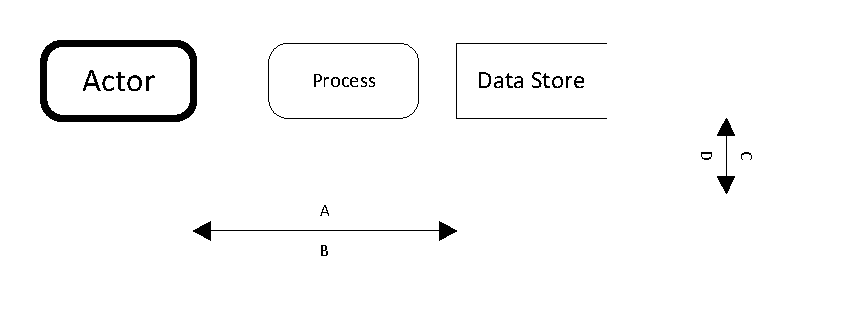
\includegraphics[keepaspectratio, width=4in]{dfd_legend.pdf}\\
\begin{itemize}
\item Actor = some user or another system that interacts with the system.
\item Process = name of some action that will be taken on the data
\item Data Store = something like a file or database that stores data
\end{itemize}
With the bidirectional arrows the data listed on above the arrow (like A) flows left-to-right, data listed below the arrow (like B) flows right-to-left, data listed to the right of the arrow (like C) flows top-to-bottom, and data listed to the left of the arrow (like D) flows bottom-to-top.

\paragraph{Context/Level 0}
~\\
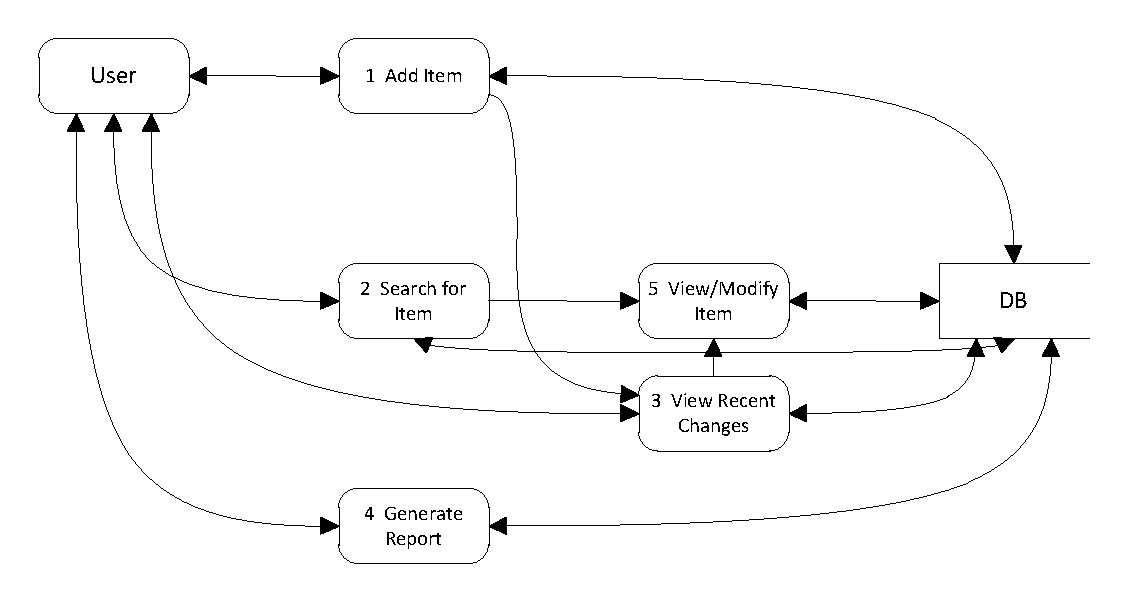
\includegraphics[keepaspectratio, width=6.5in]{dfd_context_level0.pdf}\\
~\\

\paragraph{Level 1: Add Item}
~\\
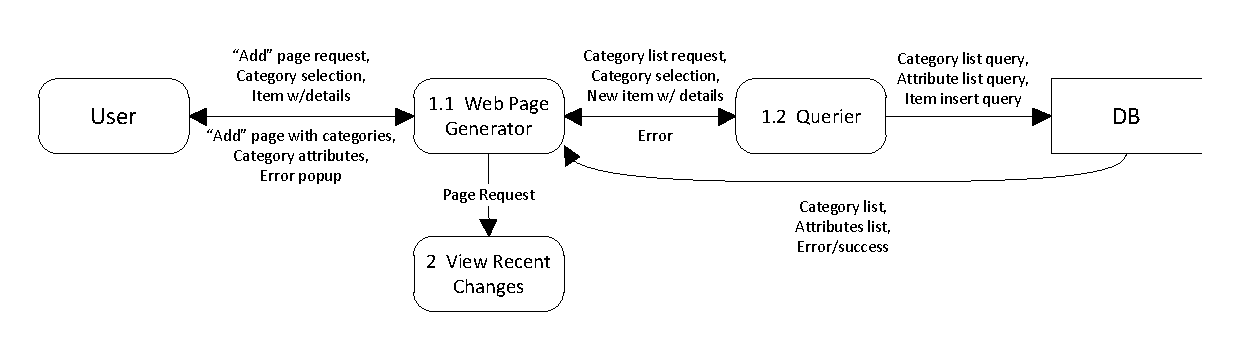
\includegraphics[keepaspectratio, width=6.5in]{dfd_level1_add_item.pdf}\\
~\\

\paragraph{Level 2: Add Item--Querier}
~\\
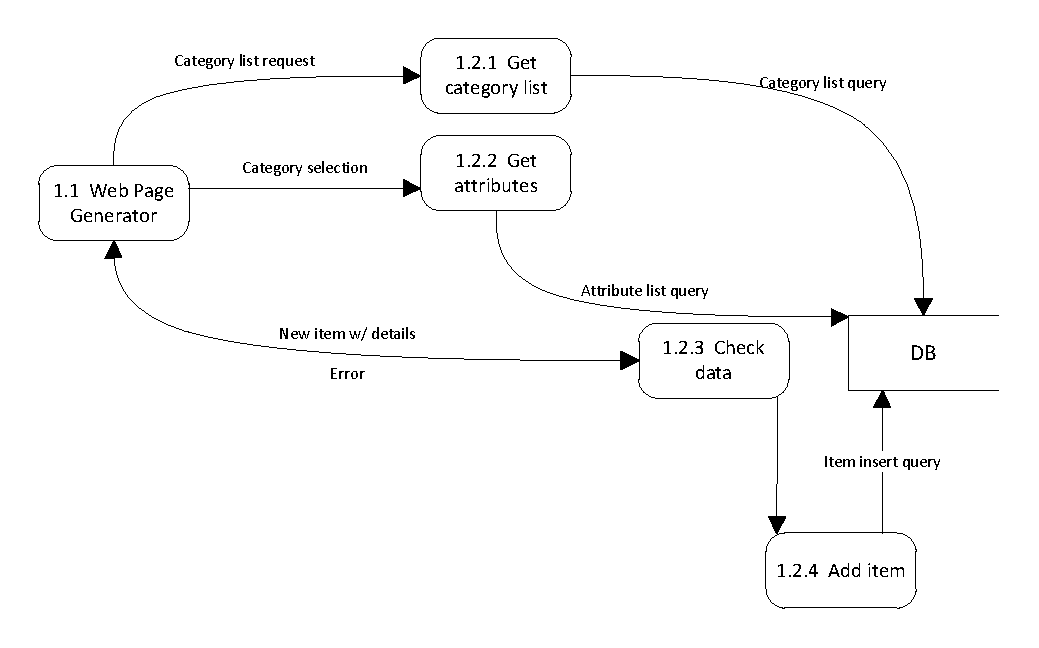
\includegraphics[keepaspectratio, width=6.5in]{dfd_level2_add_item_querier.pdf}\\
~\\

\paragraph{Level 1: Search for Item}
~\\
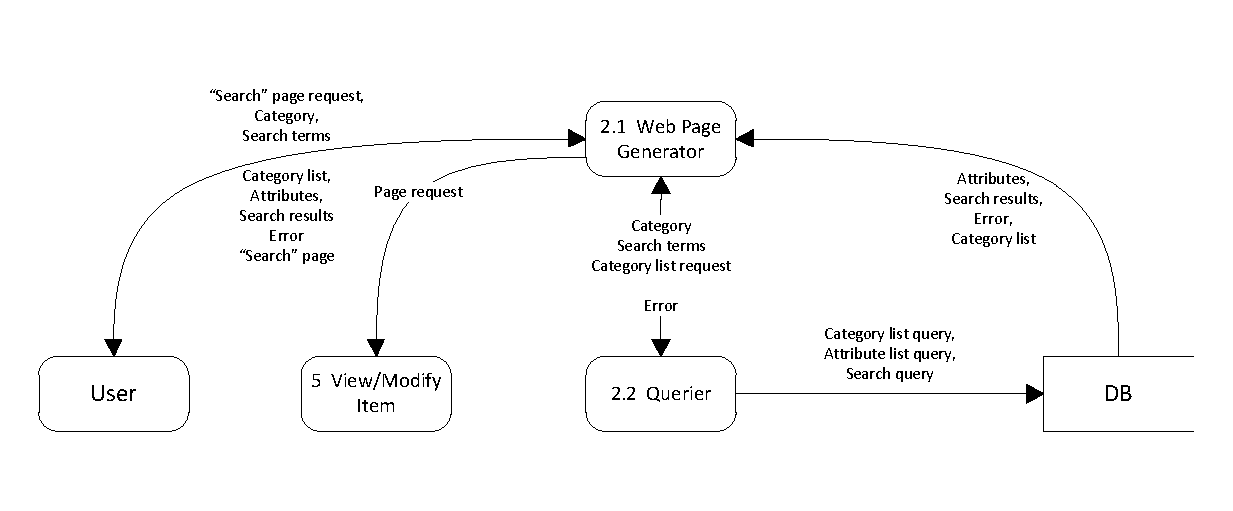
\includegraphics[keepaspectratio, width=6.5in]{dfd_level1_search_for_item.pdf}\\
~\\

\paragraph{Level 2: Search for Item--Querier}
~\\
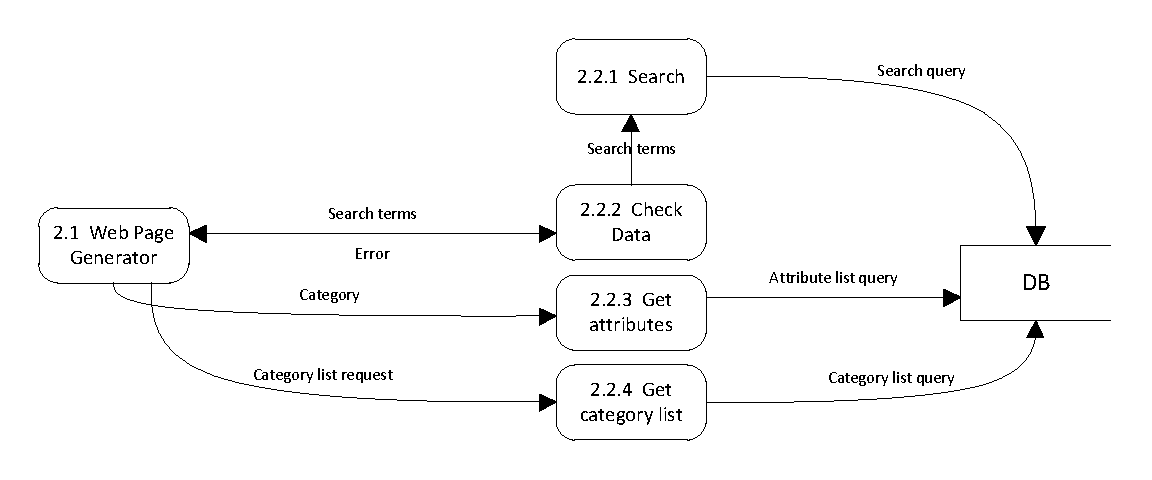
\includegraphics[keepaspectratio, width=6.5in]{dfd_level2_search_for_item_querier.pdf}\\
~\\

\paragraph{Level 1: View Recent Changes}
~\\
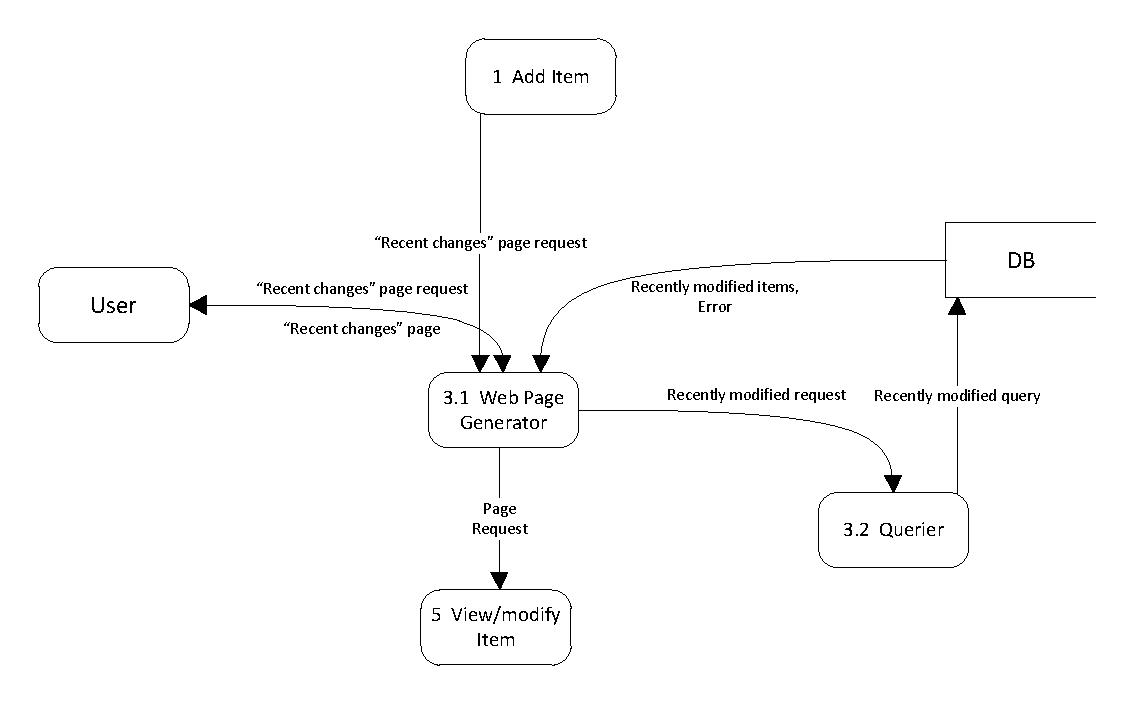
\includegraphics[keepaspectratio, width=6.5in]{dfd_level1_view_recent_changes.pdf}\\
~\\

\paragraph{Level 1: Generate Report}
~\\
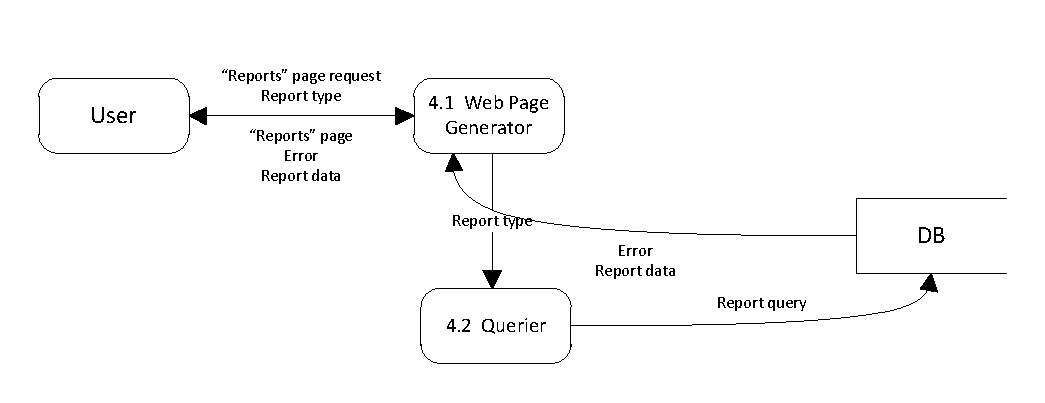
\includegraphics[keepaspectratio, width=6.5in]{dfd_level1_generate_report.pdf}\\
~\\

\paragraph{Level 1: View/Modify Item}
~\\
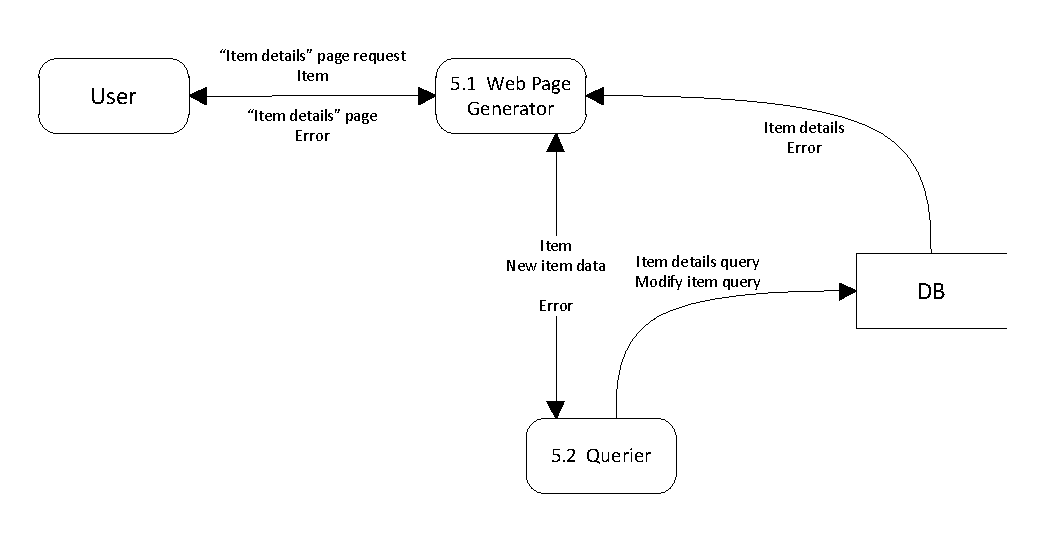
\includegraphics[keepaspectratio, width=6.5in]{dfd_level1_view_modify_item.pdf}\\
~\\

\paragraph{Level 2: View/Modify Item--Querier}
~\\
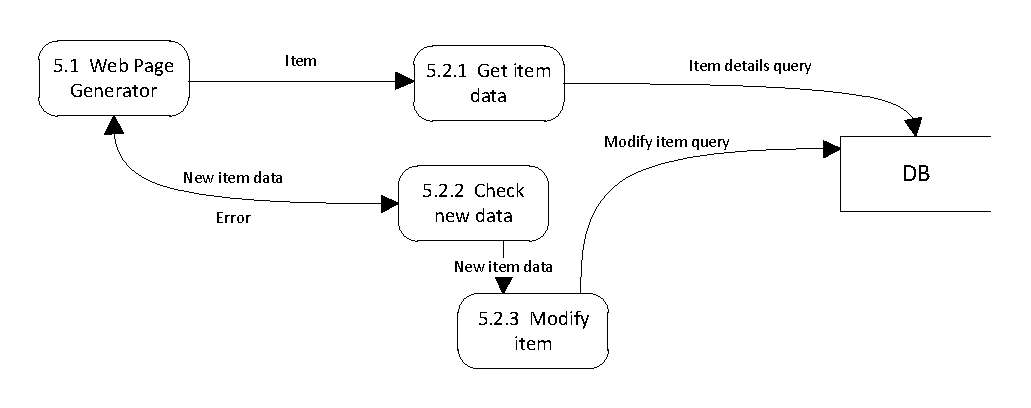
\includegraphics[keepaspectratio, width=6.5in]{dfd_level2_view_modify_item_querier.pdf}\\
~\\

\section{Index and Glossary}

\section{References}
\hangindent=1.4cm
\textbf{(1)} Leffingwell, Dean, and Don Widrig.
\emph{Managing Software Requirements: a Use Case Approach}.
Addison-Wesley, Boston,
2nd Edition,
2003.

\end{document}